\documentclass[noauthor,nooutcomes,hints,handout]{ximera}

\graphicspath{  
{./}
{./whoAreYou/}
{./drawingWithTheTurtle/}
{./bisectionMethod/}
{./circles/}
{./anglesAndRightTriangles/}
{./lawOfSines/}
{./lawOfCosines/}
{./plotter/}
{./staircases/}
{./pitch/}
{./qualityControl/}
{./symmetry/}
{./nGonBlock/}
}


%% page layout
\usepackage[cm,headings]{fullpage}
\raggedright
\setlength\headheight{13.6pt}


%% fonts
\usepackage{euler}

\usepackage{FiraMono}
\renewcommand\familydefault{\ttdefault} 
\usepackage[defaultmathsizes]{mathastext}
\usepackage[htt]{hyphenat}

\usepackage[T1]{fontenc}
\usepackage[scaled=1]{FiraSans}

%\usepackage{wedn}
\usepackage{pbsi} %% Answer font


\usepackage{cancel} %% strike through in pitch/pitch.tex


%% \usepackage{ulem} %% 
%% \renewcommand{\ULthickness}{2pt}% changes underline thickness

\tikzset{>=stealth}

\usepackage{adjustbox}

\setcounter{titlenumber}{-1}

%% journal style
\makeatletter
\newcommand\journalstyle{%
  \def\activitystyle{activity-chapter}
  \def\maketitle{%
    \addtocounter{titlenumber}{1}%
                {\flushleft\small\sffamily\bfseries\@pretitle\par\vspace{-1.5em}}%
                {\flushleft\LARGE\sffamily\bfseries\thetitlenumber\hspace{1em}\@title \par }%
                {\vskip .6em\noindent\textit\theabstract\setcounter{question}{0}\setcounter{sectiontitlenumber}{0}}%
                    \par\vspace{2em}
                    \phantomsection\addcontentsline{toc}{section}{\thetitlenumber\hspace{1em}\textbf{\@title}}%
                     }}
\makeatother



%% thm like environments
\let\question\relax
\let\endquestion\relax

\newtheoremstyle{QuestionStyle}{\topsep}{\topsep}%%% space between body and thm
		{}                      %%% Thm body font
		{}                              %%% Indent amount (empty = no indent)
		{\bfseries}            %%% Thm head font
		{)}                              %%% Punctuation after thm head
		{ }                           %%% Space after thm head
		{\thmnumber{#2}\thmnote{ \bfseries(#3)}}%%% Thm head spec
\theoremstyle{QuestionStyle}
\newtheorem{question}{}



\let\freeResponse\relax
\let\endfreeResponse\relax

%% \newtheoremstyle{ResponseStyle}{\topsep}{\topsep}%%% space between body and thm
%% 		{\wedn\bfseries}                      %%% Thm body font
%% 		{}                              %%% Indent amount (empty = no indent)
%% 		{\wedn\bfseries}            %%% Thm head font
%% 		{}                              %%% Punctuation after thm head
%% 		{3ex}                           %%% Space after thm head
%% 		{\underline{\underline{\thmname{#1}}}}%%% Thm head spec
%% \theoremstyle{ResponseStyle}

\usepackage[tikz]{mdframed}
\mdfdefinestyle{ResponseStyle}{leftmargin=1cm,linecolor=black,roundcorner=5pt,
, font=\bsifamily,}%font=\wedn\bfseries\upshape,}


\ifhandout
\NewEnviron{freeResponse}{}
\else
%\newtheorem{freeResponse}{Response:}
\newenvironment{freeResponse}{\begin{mdframed}[style=ResponseStyle]}{\end{mdframed}}
\fi



%% attempting to automate outcomes.

%% \newwrite\outcomefile
%%   \immediate\openout\outcomefile=\jobname.oc
%% \renewcommand{\outcome}[1]{\edef\theoutcomes{\theoutcomes #1~}%
%% \immediate\write\outcomefile{\unexpanded{\outcome}{#1}}}

%% \newcommand{\outcomelist}{\begin{itemize}\theoutcomes\end{itemize}}

%% \NewEnviron{listOutcomes}{\small\sffamily
%% After answering the following questions, students should be able to:
%% \begin{itemize}
%% \BODY
%% \end{itemize}
%% }
\usepackage[tikz]{mdframed}
\mdfdefinestyle{OutcomeStyle}{leftmargin=2cm,rightmargin=2cm,linecolor=black,roundcorner=5pt,
, font=\small\sffamily,}%font=\wedn\bfseries\upshape,}
\newenvironment{listOutcomes}{\begin{mdframed}[style=OutcomeStyle]After answering the following questions, students should be able to:\begin{itemize}}{\end{itemize}\end{mdframed}}



%% my commands

\newcommand{\snap}{{\bfseries\itshape\textsf{Snap!}}}
\newcommand{\flavor}{\link[\snap]{https://snap.berkeley.edu/}}
\newcommand{\mooculus}{\textsf{\textbf{MOOC}\textnormal{\textsf{ULUS}}}}


\usepackage{tkz-euclide}
\tikzstyle geometryDiagrams=[rounded corners=.5pt,ultra thick,color=black]
\colorlet{penColor}{black} % Color of a curve in a plot



\ifhandout\newcommand{\mynewpage}{\newpage}\else\newcommand{\mynewpage}{}\fi


\author{Jenny Sheldon \and Bart Snapp}

\title{Line art}

\begin{document}
\begin{abstract}
  We draw curves with lines.
\end{abstract}
\maketitle

\begin{listOutcomes}
\item Understand how to draw an envelope of tangents by hand.
\item Understand how to draw a sequence of envelopes of tangents with
  increasing precision.
\item Find and prove a rule.
\end{listOutcomes}


Get out a piece of paper, a ruler, and a writing utensil. Really, do
it!  Seriously! Now draw two lines that come to a point:
\[
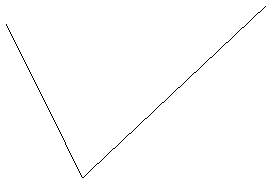
\includegraphics{mesh0.pdf}
\]
Next, take both of those lines and mark the midpoints. Connect the
midpoints with a line:
\[
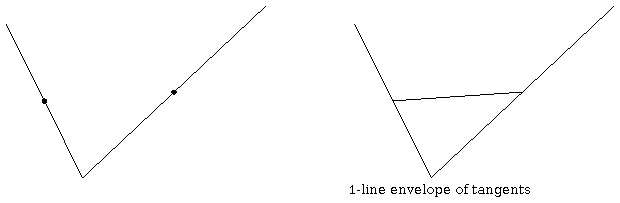
\includegraphics{mesh1.pdf}
\]
Each original line is now divided into two segments. Mark the
midpoints of those segments and cross-connect them:
\[
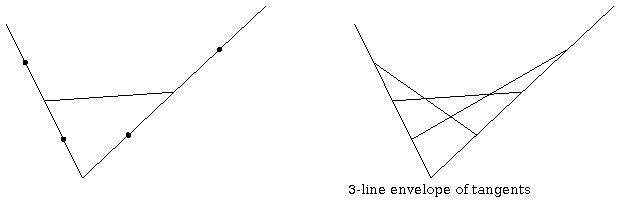
\includegraphics{mesh2.pdf}
\]
If you continue this cross-connecting process, you'll get groovy pictures like these:
\[
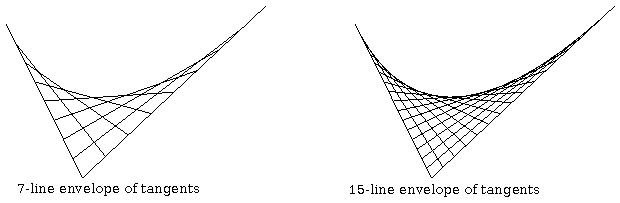
\includegraphics{mesh3.pdf}
\]
Over 2000 years ago, Apollonius of Perga explained why the curve
formed by these segments is a \index{parabola}parabola. Today we call
what we just drew an \textit{envelope of tangents}\index{envelope of
  tangents}.  If we cross-connect $n$ pairs of lines we'll call this
an \textit{$n$-line envelope of tangents}.




\paragraph{B\'ezier curves}

While some of us like pointy drawings, others like smooth drawings. To
make smooth drawings, we'll need the help of $\textit{Pierre
  B\'ezier}$, pronounced ``beh-zeeayr.'' Here is the deal.  Pierre
B\'ezier was an engineer with the Renault car company in the
1960's. He needed a convenient way to draw curves, a way that would
allow curves to be:
\begin{enumerate}
\item Easy to render---meaning easy for a computer (or person!) to
  reproduce the curve described by the artist.
\item Easy to transform---meaning easy to manipulate the curve with
  geometric transformations.
\item Easy to draft---meaning easy for an artist to shape a desired
  curve.
\end{enumerate}
Given two end-points, B\'ezier devised a way to work with
curves via a \textit{node} and two
\textit{control points}:\index{node}\index{control-point}
\[
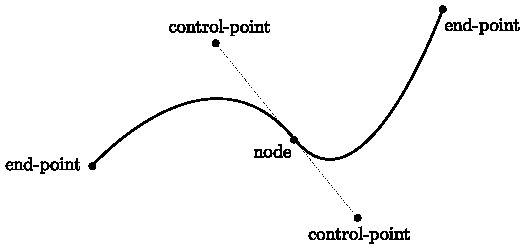
\includegraphics{bezier.pdf}
\]
With the end points remaining fixed, the artist can move the node and
control points to change the way the curve looks.  But how do those
so-called control points actually control the way the curve looks?
Well, the end points, node, and control points define a polygonal path:
\[
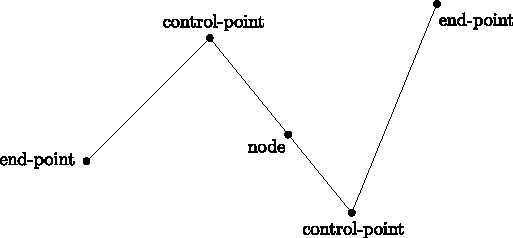
\includegraphics{bezierPoly.pdf}
\]
This polygonal path in turn gives an envelope of tangents, which then gives
the desired curve:
\[
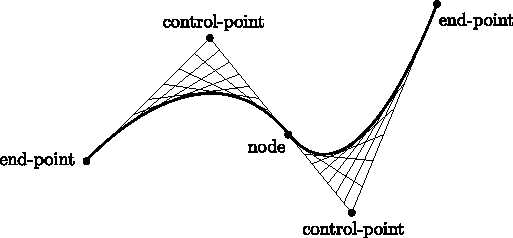
\includegraphics{bezierMesh.pdf}
\]
While this may seem all fancy and highfalutin, it is the essence of
B\'ezier's method for drawing curves.  It has become so popular that
this is basically how curves are currently drafted using vector
graphics programs such as \textit{Adobe Illustrator} and
\textit{Inkscape}. Why are B\'ezier curves so popular? We'll see that
they satisfy the requirements above quite well.

\paragraph{Easy to render}
A computer does not draw the parabola via an envelope of
tangents---however, the process we use above can be done by hand. The
key point is that one can obtain an arbitrary amount of smoothness to
the hand-drawn curve by simply adding  more lines to the envelope of tangents.



\paragraph{Easy to transform}
Each curve is completely determined by the polygonal path from the
first end point to first control point to the node to the other
control point and the final end point. Hence, if I simply handed you
five points:
\[
(1,4)\to (4,2)\to (6,6)\to (7,8)\to(9,4)
\]
you can then draw a curve and tell someone else how to draw the exact
same curve. Moreover, you could transform the entire curve merely by
transforming those five points.



\paragraph{Easy to draft}
Of course, as you are aware, most graphic artists don't think much
about coordinates and yet are still able to draw B\'ezier curves with
impunity. This is really the genius of B\'ezier's method. By fixing
the end points, one only need to know the position of the node and the
control points. So by using a mouse, an artist can move the
control points and node to get a plethora of interesting curves.




\mynewpage






\begin{question}
  CAREFULLY draw a $15$-line envelope of tangents BY HAND. Use a
  RULER. Make it BIG, take up the whole page!
  \begin{freeResponse}
    NOT DONE
  \end{freeResponse}
\end{question}
\mynewpage





\begin{question}
  Suppose you are helping someone build an archway for their home from
  a board that is $12''\times 42''$:
  \begin{center}
    \begin{tikzpicture}[geometryDiagrams,scale=.8]
      \begin{scope}
        \clip(-2.2in,0) rectangle (2.2in,1.3in);
        \draw[dashed,thin] (0,0) ellipse (1.9in and 1in);
      \end{scope}
      \draw (-1.9in,0in) -- (-2.1in,0in) -- (-2.1in,1.2in) -- (2.1in,1.2in) -- (2.1in,0in) -- (1.9in,0in);
      \draw[dashed, thin] (-1.9in,0in) -- (1.9in,0in);
      \draw[decoration={brace,raise=.2cm,mirror},decorate,thin] (2.1in,0in)--(2.1in,1.2in);
      \draw[decoration={brace,raise=.2cm},decorate,thin] (-2.1in,1.2in)--(2.1in,1.2in);
      \draw[decoration={brace,raise=.2cm,mirror},decorate,thin] (-1.9in,0in)--(1.9in,0in);
      \draw[|-|,thin] (0in,.05in)--(0in,.95in);
      \node[below] at (0,-.1in) {$38''$};
      \node[above] at (0,1.3in) {$42''$};
      \node[right] at (2.2in,.6in) {$12''$};
      \node[right] at (0in,.5in) {$10''$};
        \end{tikzpicture}
    \end{center}
  \begin{enumerate}
  \item STRING:
    Use the fact that 
    \[
    \mathrm{distance}(f_1,m) + \mathrm{distance}(f_2,m) =
    \mathrm{distance}(f_1,M) + \mathrm{distance}(f_2,M)
    \]
    to deduce \textbf{one} of the following:
    \[
    a^2 = b^2 + c^2 \qquad\text{or}\qquad
    b^2 = a^2+c^2 \qquad\text{or}\qquad c^2 = a^2 + b^2
    \]
    REPRODUCE the drawing above including the CORRECT MEASUREMENTS for
    $c$. Show all work and explain your reasoning.


  \item It turns out that your friend has Laser cutter that can be
    controlled by \snap\ blocks. To draw an ellipse in \snap\ like
    this one:
    \begin{center}
        \begin{tikzpicture}[geometryDiagrams,scale=.8]
          \draw (0,0) ellipse (2in and 1in);
          \draw[->,thin] (0in,-1.5in) -- (0in,1.5in);
          \draw[->,thin] (-2.5in,0in) -- (2.5in,0in);
          \filldraw[black] (2in,0) circle (2pt) node[above right] {(a,0)};
          \filldraw[black] (0,1in) circle (2pt) node[above right] {(0,b)};

          \filldraw[black] (1.73in,0in) circle (2pt) node[below left] {(c,0)};
          \filldraw[black] (-1.73in,0in) circle (2pt) node[below right] {(-c,0)};

          \draw[dashed,thin] (-1.73in,0in) -- (.9in,.89in);
          \draw[dashed,thin] (1.73in,0in) -- (.9in,.89in);

          \node at (-.75in,.5in) {$X$};
          \node at (1.2in,.35in) {$Y$};
          
          \filldraw[black] (.9in,.89in) circle (2pt);
        \end{tikzpicture}
      \end{center}
    use
    \[
    x = a\sin(\theta) \qquad\text{and} \qquad y= b\cos(\theta)
    \]
    Using the DEFINITION of an ellipse, explain WHY the equations
    above DRAW an ellipse and not some other oval.
    \begin{hint}
      This will help you on the way.
      \begin{itemize}
      \item Write the sum of distances between the foci and $(x,y)= (a\sin(\theta),b\cos(\theta))$.
      \item Recall that $\cos^2(\theta) = 1-\sin^2(\theta)$.
      \item Use the fact from the previous part.
      \end{itemize}
    \end{hint}  
    \item Use an envelope of tangents to draw this arch.
    
  \end{enumerate}

\end{question}
\mynewpage


%% BADBAD REWRITE IN TERMS OF SMOOTHING
\begin{question}
  Suppose you have a $7$-line envelope of tangents. However, it is not
  SMOOTH enough. To SMOOTH the curve, add an additional $8$ lines to
  make a $15$ line envelope of tangents. Check it out:
  \begin{center}
  ORGINAL 7-LINE NEEDS TO BE HERE  \fbox{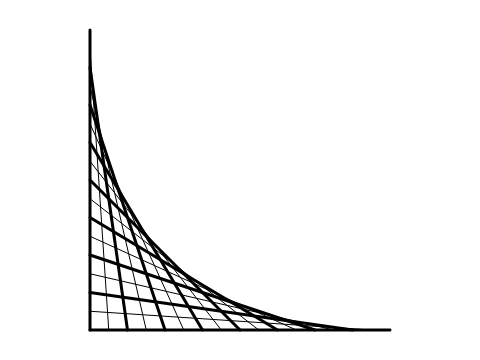
\includegraphics[width=.3\textwidth]{7-15-lineOfTanEG.png}}
  \end{center}
  Can you figure out how to smooth curves drawn with envelopes of
  tangents?
  \begin{enumerate}
    \item Extend an $8$-line envelope of tangents by halving all of
      the ``squares.''  Show off your work by displaying a SCRIPT and
      a STAGE.
    \item Extend a $9$-line envelope of tangents by halving all of the
      ``squares.''  Show off your work by displaying a SCRIPT and a
      STAGE.
    \item Give a general rule for halving all of the ``squares'' of an
      $n$-line envelope of tangents. EXPLAIN WHY the general rule works.
  \end{enumerate}
  As a gesture of friendship, I offer this useful script:
  \begin{center}
    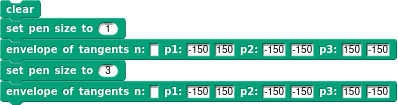
\includegraphics{genericExtendedEnvelopeOfTan.png}
  \end{center}
  \begin{freeResponse}
    \begin{enumerate}
    \item Here is my SCRIPT and my STAGE:
      \begin{center}
        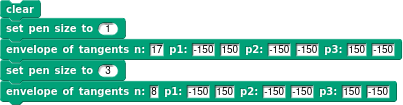
\includegraphics[width=.3\textwidth]{8-17-lineOfTanScript.png}\qquad\fbox{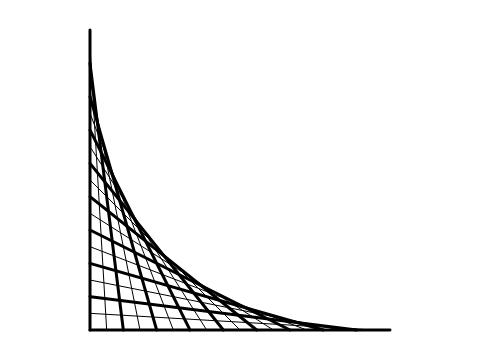
\includegraphics[width=.3\textwidth]{8-17-lineOfTanStage.png}}
      \end{center}
    \item Here is my SCRIPT and my STAGE:
      \begin{center}
        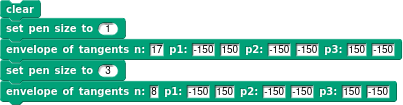
\includegraphics[width=.3\textwidth]{8-17-lineOfTanScript.png}\qquad\fbox{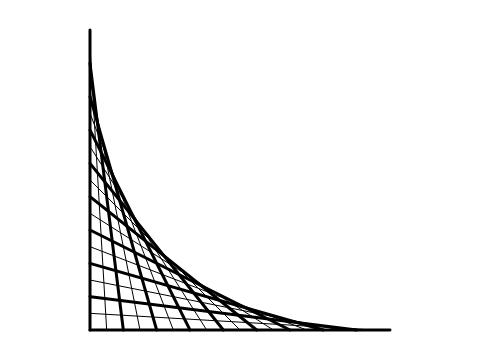
\includegraphics[width=.3\textwidth]{8-17-lineOfTanStage.png}}
      \end{center}
    \item To halve the ``squares'' of an $n$-line envelope of
      tangents, draw an $(2n+1)$-line envelope of tangents. This works
      because with $n$ lines, there are $n+1$ gaps and $n + n+1 =
      2n+1$.
    \end{enumerate}
  \end{freeResponse}
\end{question}




%% \mynewpage
%% \begin{question}
%%   Let's continue doing what we did in the last problem.
%%   \begin{enumerate}
%%   \item Explain how to ``third'' all of the ``squares'' of an envelope
%%     of tangents. Along with your EXPLANATION, show one STAGE as an
%%     example.
%%   \item Explain how to ``quarter'' all of the ``squares'' of an
%%     envelope of tangents. Along with your EXPLANATION, show one STAGE
%%     as an example.
%%   \item Given an $n$-line envelope of tangents, explain how to
%%     ``$i$-th'' every square. EXPLAIN why this method works.
%%   \end{enumerate}
%%   \begin{freeResponse}
%%     \begin{enumerate}
%%     \item To ``third'' all of the ``squares'' of an $n$-line envelope
%%       of tangents, draw a $(3n+2)$-line envelope of tangents.
%%       \begin{center}
%%         \fbox{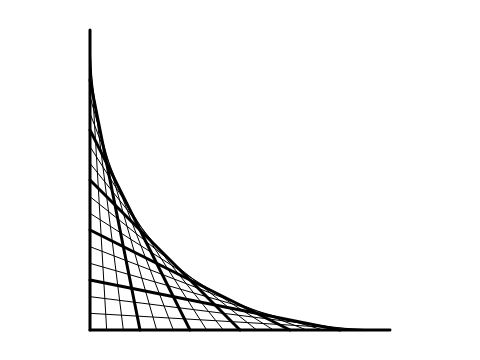
\includegraphics[width=.3\textwidth]{5-17-lineOfTanEG.png}}
%%       \end{center}
%%       This works because with $n$ lines, there are $n+1$ gaps, and in
%%       each of these gaps there are $2$ new lines, so
%%       \[
%%       n + (n+1)\cdot 2  = 3n+2.
%%       \]
%%     \item To ``quarter'' all of the ``squares'' of an envelope of
%%       tangents, draw a $(4n+3)$-line envelope of tangents.
%%       \begin{center}
%%         \fbox{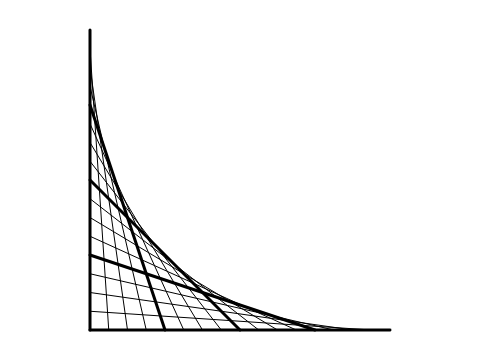
\includegraphics[width=.3\textwidth]{3-15-lineOfTanEG.png}}
%%       \end{center}
%%       This works because with $n$ lines, there are $n+1$ gaps, and in
%%       each of these gaps there are $3$ new lines, so
%%       \[
%%       n + (n+1)\cdot 3  = 4n+3.
%%       \]
%%     \item To ``$i$-th'' every square of an $n$-line envelope of
%%       tangents, draw a $(i\cdot n+i-1)$-line envelope of
%%       tangents. This works because with $n$ lines, there are $n+1$
%%       gaps, and in each of these gaps there are $(i-1)$ new lines, so
%%       \[
%%       n + (n+1)\cdot (i-1)  = i\cdot n+i-1.
%%       \]
      
%%   \end{enumerate}
%%   \end{freeResponse}
%% \end{question}
\end{document}
